\documentclass[twocolumn]{IEEEtran}
\usepackage{url}
\usepackage{amsmath}
%\let\proof\relax \let\endproof\relax
\usepackage{amsthm}
\usepackage[linesnumbered,ruled]{algorithm2e}
\usepackage{verbatim}
\usepackage{graphicx}
\usepackage{subfigure}
\newtheorem{theorem}{Theorem}
\newtheorem*{theorem_nn}{Theorem}
\newtheorem{lemma}{Lemma}
\newtheorem{definition}{Definition}
\newtheorem{corollary}{Corollary}
\newtheorem{proposition}{Proposition}
\newtheorem{conjecture}{Conjecture}
\newtheorem{prob}{Problem}
\newtheorem{lemm}{Lemma}
\theoremstyle{definition}
\newtheorem{IP}{Integer Program}
\newtheorem{remark}{Remark}
\newtheorem{deff}{Definition}
\newtheorem{claim}{Claim}
\newtheorem{examp}{Example}
\newtheorem{prop}{Property}
\newtheorem{propp}{Proposition}
\newtheorem{assume}{Assumption}
\graphicspath{{figures/}}
\usepackage{amsmath}
\usepackage{mathrsfs}
\usepackage{amssymb}
\usepackage{booktabs}
\usepackage{changepage}
%\newcommand{\shrinkfig}{\vspace{-0.5cm}}
\DeclareMathOperator*{\argmax}{arg\,max}

\usepackage{tikz}
\usetikzlibrary{arrows}

\begin{document}

\section{Edge-clustering coefficients}
Let $G = (V, E)$ be an undirected, unweighted graph.
$N(u) = \{ w \in V : d(u,w) = 1 \}$, where $d(u,w)$ is
the hop distance between $u,w$.
\begin{definition}[Local clustering coefficient of an edge]
  Let $(u,v) \in E$. Then
    \[ c(u,v) = \frac{ | N(u) \cap N(v) | }{ | N(u) \cup N(v) \backslash \{u, v \} | }. \]
\end{definition}

This definition is similar to the one in \cite{}, which replaces
the denominator above with $\min \{ |N(u)| - 1, |N(v)| - 1\}$.

\subsection{Longer cycles}
\section{Edge-clustering in Multiplex networks}
Let $\mathscr{G} = ( G_\alpha = (V, E_\alpha) )_{\alpha \in \Lambda} $ be a node-aligned multiplex network (that is, each layer of the multiplex contains the same vertices).
Consider an edge in layer $\gamma$, 
specified by $((u,v), \gamma)$, where $u,v \in V$.
Then can define edge-clustering coefficients 
\begin{definition}
  \[ c_{\alpha,\beta}( (u,v), \gamma )  = \frac{ w_{\alpha \beta \gamma} \left|N_{\alpha}(u) \cap N_{\beta}(v) \right| }{ \left| N_\alpha(u) \cup N_\beta(v) \backslash \{u, v\} \right|  }. \]

\begin{figure}
  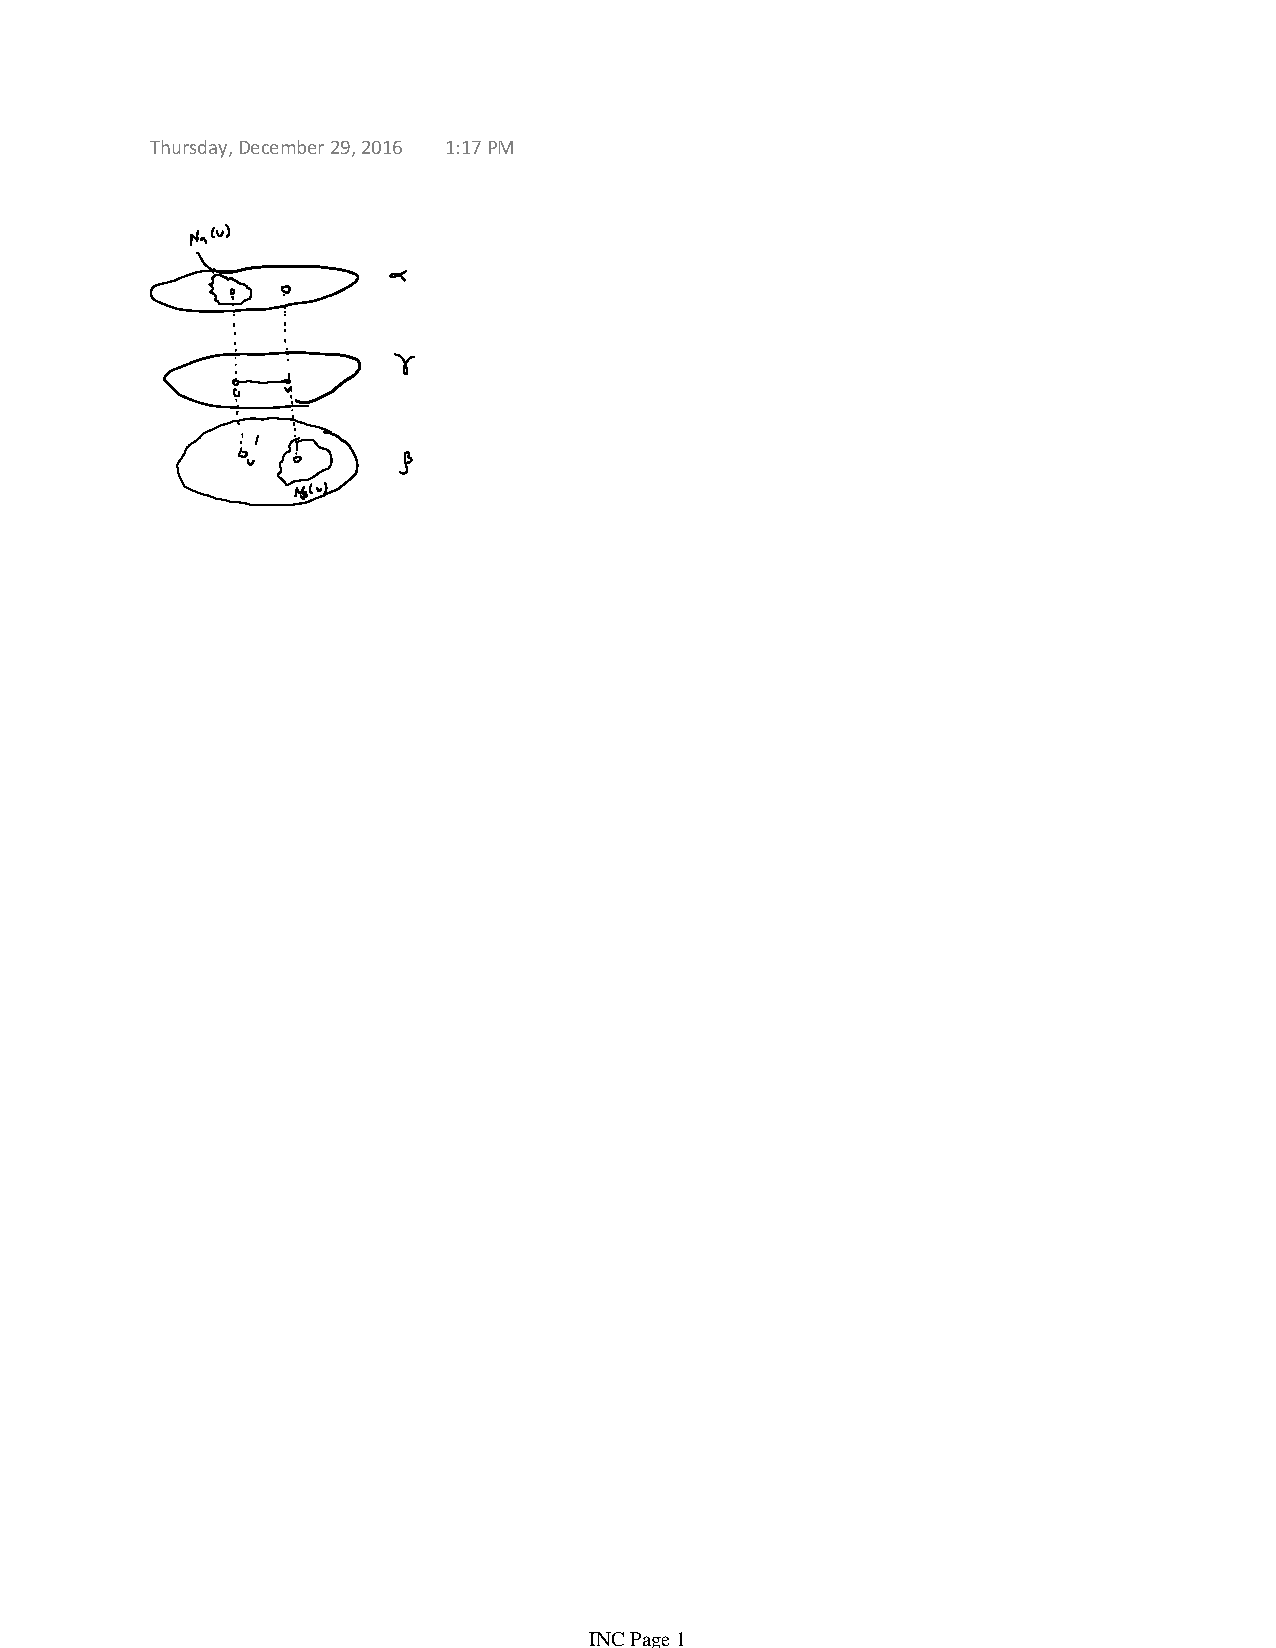
\includegraphics{fig1}
\end{figure}
\end{definition}
\section{Edge-clustering in Multilayer network}
\end{document}
